


\section{Experiments}

To evaluate the effectiveness of our approach, we conduct series of comparative test and ablation study on two datasets, YouTubeVOS \cite{xu2018Youtube} and DAVIS \cite{davis_2017} under different settings.
%We test on two datasets, YouTubeVOS \cite{xu2018youtube} and DAVIS \cite{davis_2017}, to compare the proposed STSENet with state-of-the-art methods. %Several ablation studies are conducted to prove the effectiveness of spatial details and temporal information in video inpainting.
%\subsection{Experimental Settings}

\noindent \textbf{Mask Setting.} Considering different real-world applications, we test four kinds of mask settings in this paper. 
They are different in shapes and positions of the missing regions. 
%The first and the second settings aims to recover rectangular regions, which are common in watermark removal.
(1) \emph{Fixed square mask.} The size and position of the missing square region are fixed through the whole video. 
(2) \emph{Moving square mask.} The position and size of the square mask change over frames. 
(3) \emph{Free-from mask.} We apply irregular mask which imitates hand-drawn masks on each frame, following \cite{liu2018partialinpainting}. 
(4) \emph{Foreground object mask}. This type of mask is defined to line out foreground objects in videos and used for testing object removal.

\noindent\textbf{Dataset.} 
YouTubeVOS and DAVIS are widely used for evaluating video inpainting results in recent studies.
YouTubeVOS consists of 4,453 video clips that contain more than 70 categories of common objects. 
The videos are split into three parts, 3,471 for training, 474 for validating, and 508 for testing. Since YoutubeVOS has no dense foreground mask annotations, we only use it for evaluation of mask settings (1), (2), and (3). 
% 
DAVIS dataset contains 90 video sequences that are annotated with foreground object masks and 60 unlabeled videos for training.


\dlt{
is for video object segmentation containing 150 video clips, among which 60 randomly sampled clips are for testing of object removal. And the rest part is used for training.
The videos are complex with occlusions, fast motion, and various objects. }

\noindent \textbf{Implementation details and Evaluation Metrics.} 
For all the mask settings, the video frames are resized into $256\times256$. The detailed training strategies are explained in the supplementary file. 
Different data preparations and evaluation metrics are applied according to mask settings.

\noindent (a) We randomly generate masks for training videos in terms of mask settings (1), (2), and (3).  
Three commonly-used metrics, including structural similarity index (SSIM) \cite{wang2004image}, peak signal-to-noise ratio (PSNR), and Fr{\'e}chet Inception Distance (FID) \cite{heusel2017gans} are used to quantitatively evaluate the performance of our method. 

\noindent (b) For mask setting (4), we prepare masks of random shapes and motions to synthesize the foreground object masks in the training stage. The network is first trained on the YoutubeVOS dataset and then finetuned on DAVIS. Since there is no ground truth available for this setting, we conduct a user study for video foreground object removal.  

 
 
  
\dlt{Adam optimizer  with $\beta=(0.9, 0.999)$.
The learning rate is set to $1e-4$ for $N^E$ and $G^F$ and $1e-5$ for $D^E$. 
Then, the TexNet is trained with learning rate of $1e-4$ for $G^I$, and $4e-4$ for $D^I$. Finally, we fix the former parts and train the temporal ensemble module with the learning rate of $1e-4$. We do not use weight decay in training.
As for the hyper-parameters, $\lambda_1=10.0,\lambda_2=5.0, \lambda_3=0.1$.}

 
\begin{figure*}[t]
	\centering
	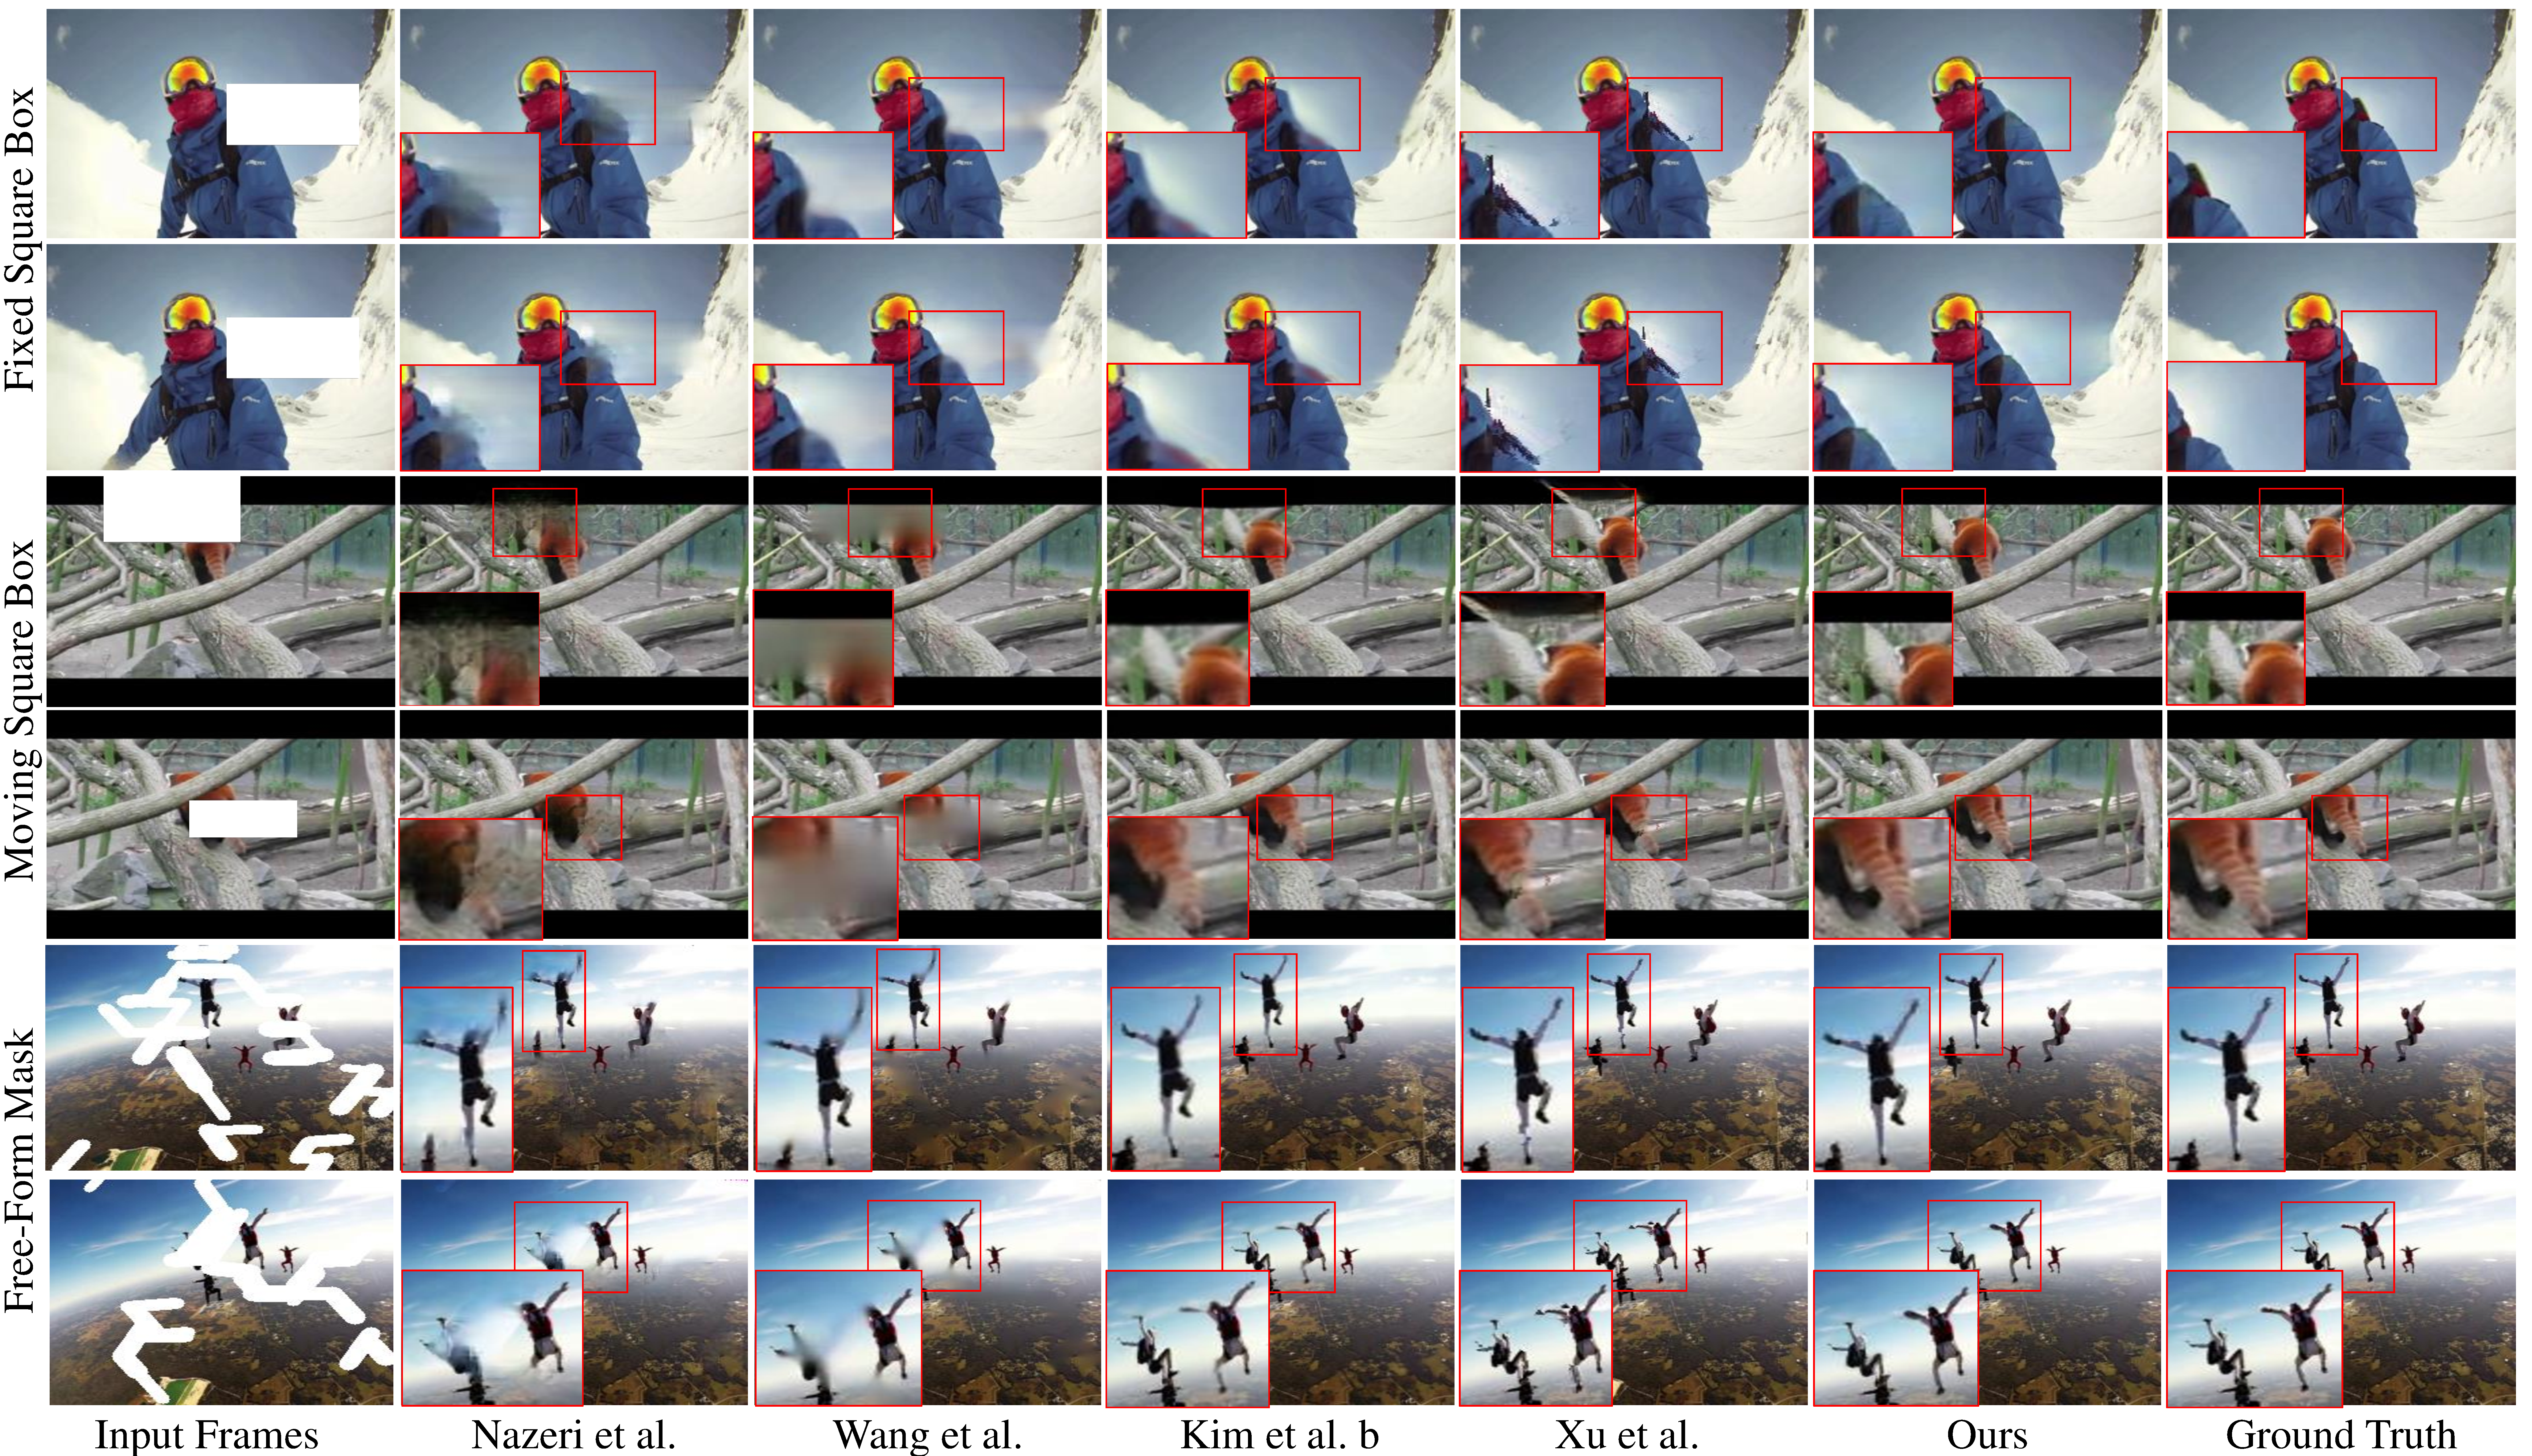
\includegraphics[scale=0.127]{viszong} % Reduce the figure size so that it is slightly narrower than the column. Don't use precise values for figure width.This setup will avoid overfull boxes. 
	\caption{Comparison on YouTubeVOS.  Our method produces more complete and finer structure than other methods.  }
	\label{viszong}
\end{figure*}


\subsection{Main Results on Video Inpainting}

We compare with four state-of-the-art inpainting methods for the first three mask settings on the YouTubeVOS dataset. %The masked videos are used as testing data.
%
We train \cite{nazeri2019edgeconnect,Xu_2019_CVPR} using their codes and re-implement \cite{wang2019video} according to their paper. As for \cite{Kim_2019_CVPR1}, we use the officially provided model since there is no available training codes.

The quantitative results and inference speeds are reported in Table~\ref{tab:sem}.
It shows that our method outperforms state-of-the-art methods on the three metrics, demonstrating the effectiveness of introducing structure guidance into video inpainting.
Moreover, our method is also very efficient, e.g. twice faster than \cite{Kim_2019_CVPR1} and four times faster than \cite{Xu_2019_CVPR}. 
%
Some inpainting examples are shown in Fig.~\ref{viszong}.
Compared with existing methods, the inpainting results predicted by our method are more realistic with finer details. 
We can observe that the frames completed using our method contain more sharper object boundaries. This is achieved by the effectiveness of structure information in video inpainting.
%
When looking at two neighboring frames in each video, it can be seen that our method produces more temporally smooth results. More comparisons can be found in the supplementary video.




Comparing with the 2D image inpainting method~\cite{nazeri2019edgeconnect} which also predicts edges to represent the structure, our method greatly increases the completion performance by leveraging neighboring frames to complete edges and synthesize textures. 
%
It demonstrates that our method is not a naive extension to utilize structure information in video inpainting.
This also indicates that structure clues can bring strong promotion to video inpainting.

%% Time performance analysis 

 

\dlt{
Specifically, the additional time cost brought by edge enhancement is negligible.
%
When the flow inpainting module is removed in SOVI, the inference speed is almost twice faster, and our performance is still competitive.
}
%





\subsection{Results on Object Removal}


In regard to the fourth setting that aims to remove undesired objects in videos, there is no ground truth for quantitatively evaluation. Therefore,
we conduct a user study on the DAVIS dataset to evaluate the visual quality of our method, comparing with four methods \cite{nazeri2019edgeconnect,wang2019video,Kim_2019_CVPR1,Xu_2019_CVPR}.
%
In each test, we show three videos to the subject at the same time. The original video with red masks indicating objects to remove is shown in the middle, while the inpainting results of our method and one of the other four method are shown on the two sides in a random order.
%  
The subjects can watch the videos repeatedly to better evaluate the differences.
For each video triplet, the subject is asked to choose which inpainting video is preferred.
40 subjects participated our user study. 
Each participant watched averagely 20 triplets. 
Therefore, each pair of methods is compared about 200 times.
%Each method is compared about 200 times.

%
\begin{figure}[!t]
	\centering
	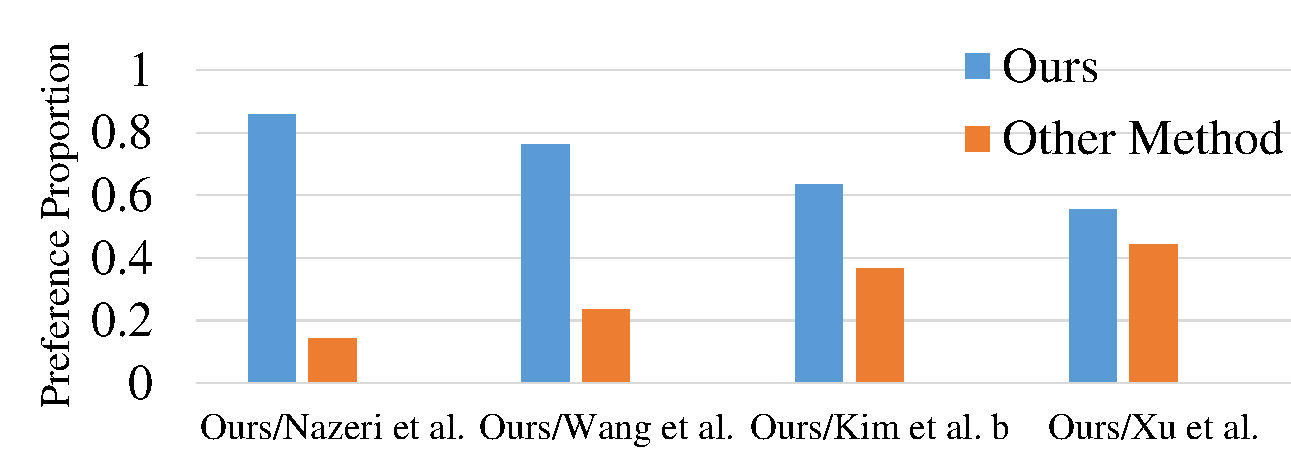
\includegraphics[width=1.0\columnwidth]{userstudy} % Reduce the figure size so that it is slightly narrower than the column. Don't use precise values for figure width.This setup will avoid overfull boxes. 
	\caption{Results of user study.}
	\label{userstudy}
\end{figure}

%
\begin{figure}[!h]
	\centering
	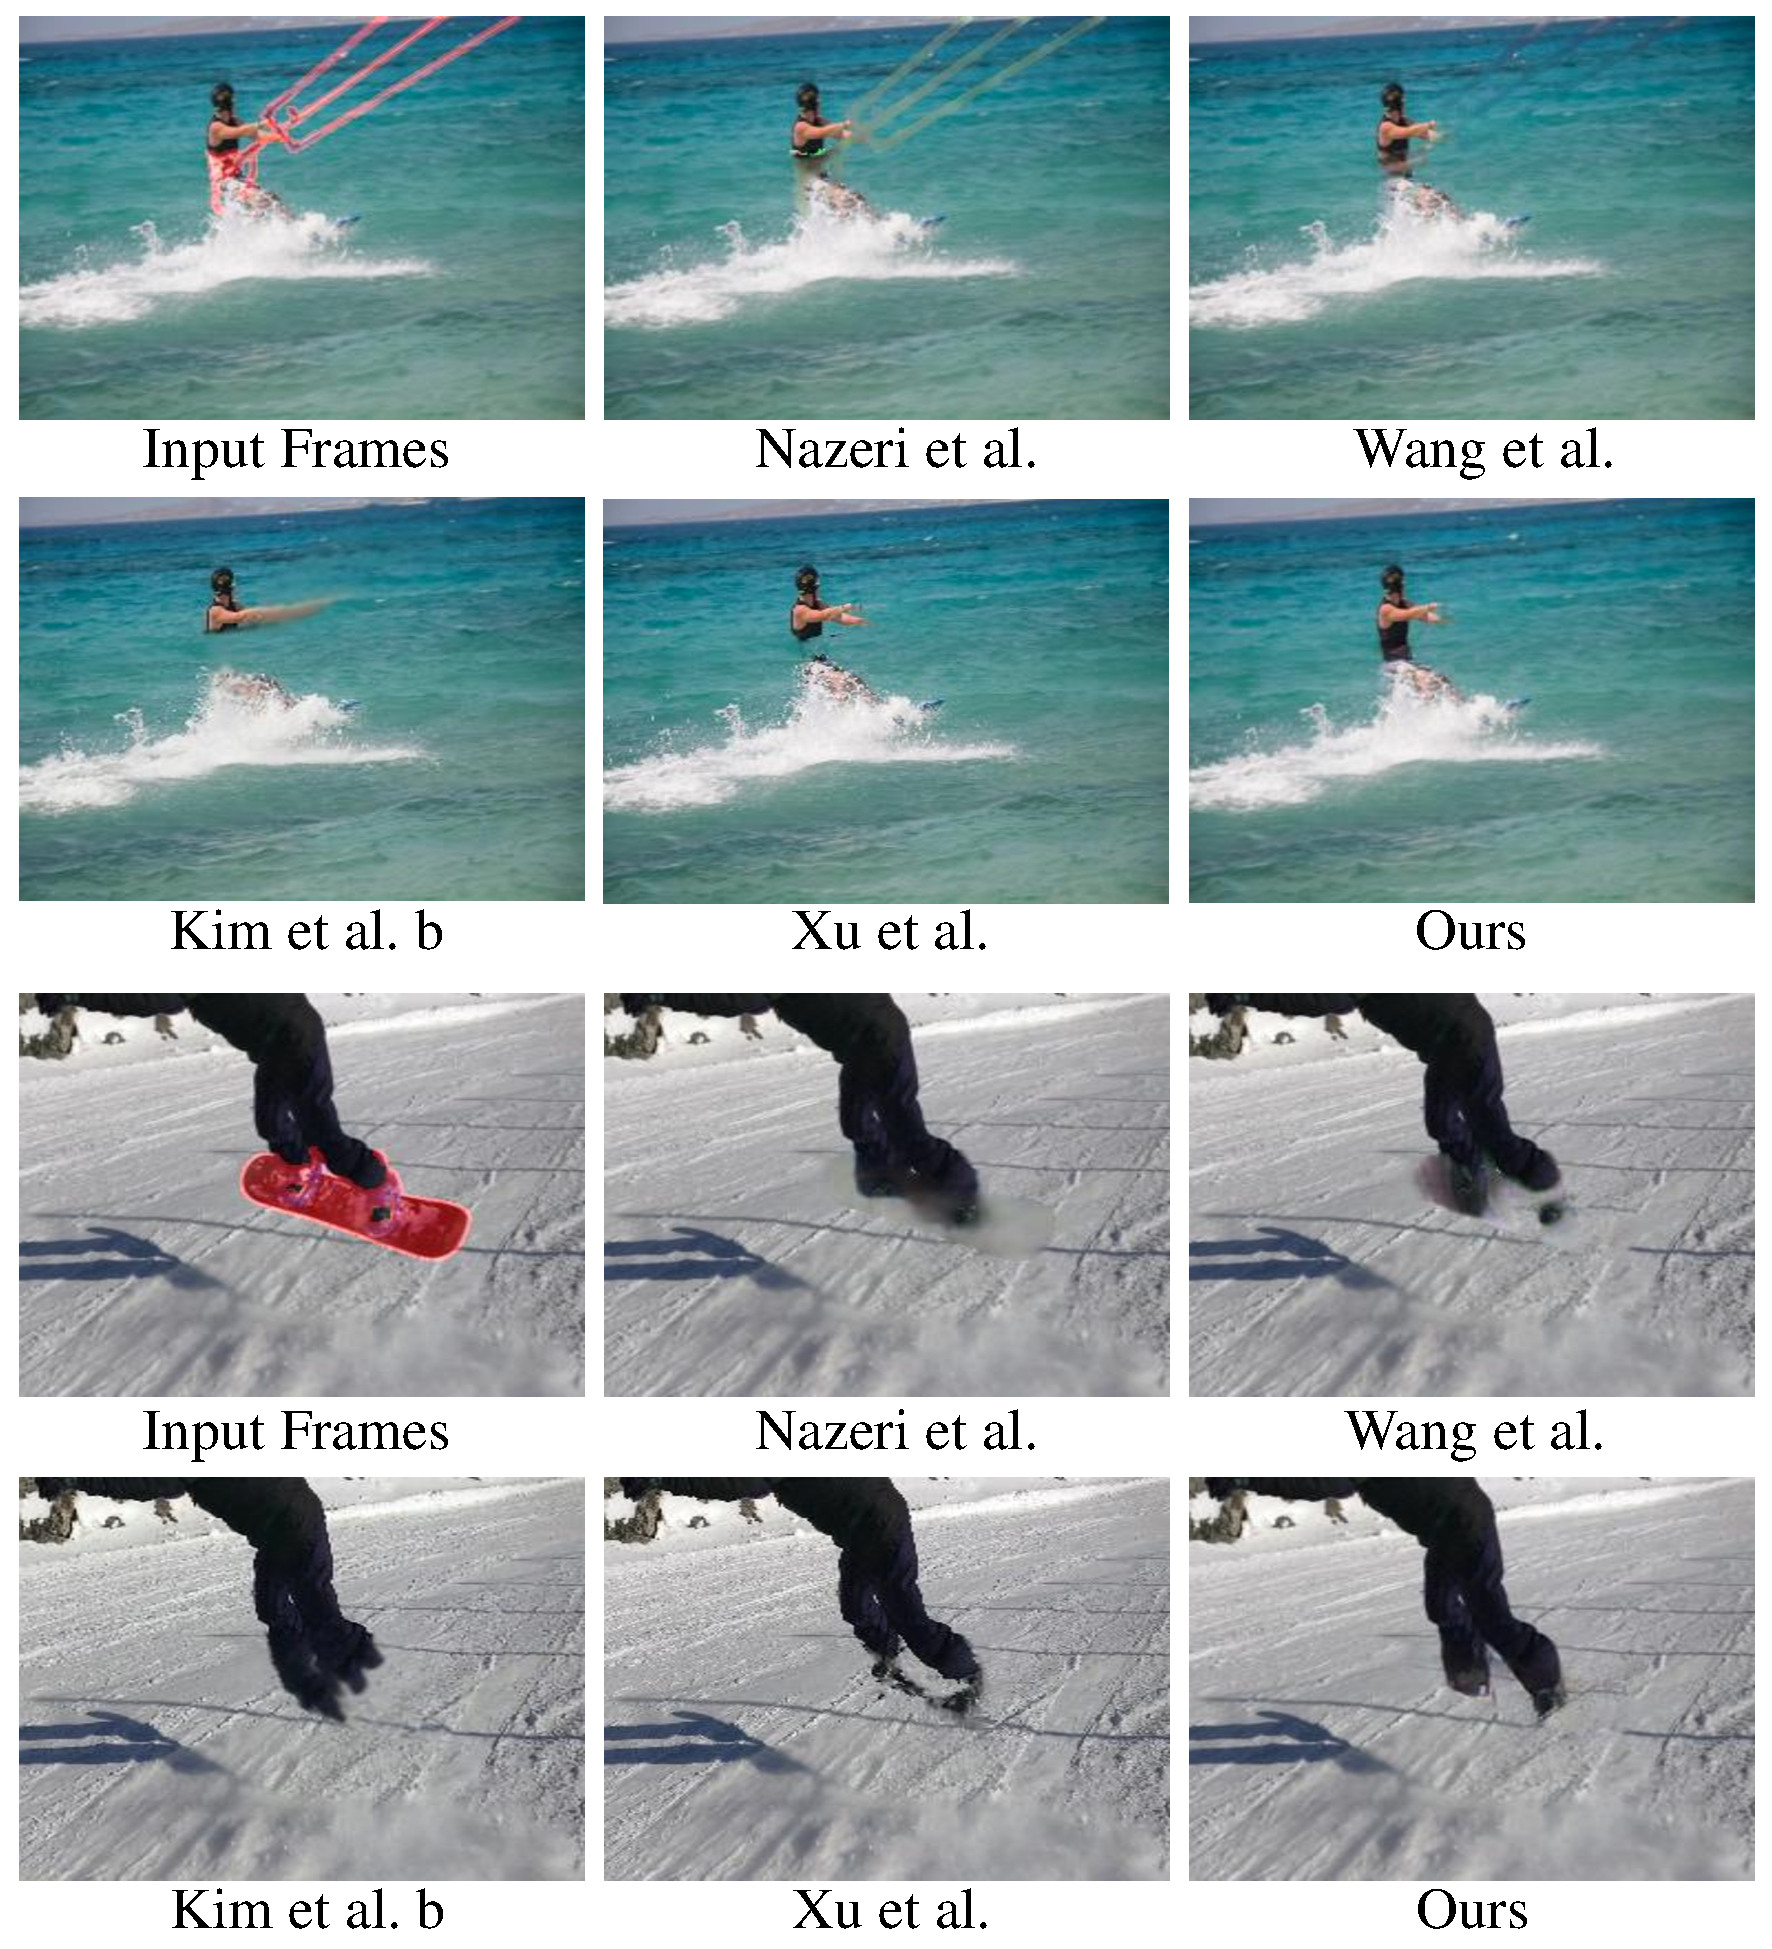
\includegraphics[width=1.0\columnwidth]{vis_forg} % Reduce the figure size so that it is slightly narrower than the column. Don't use precise values for figure width.This setup will avoid overfull boxes. 
	\caption{Results of object foreground removal. The red masks in input frames indicate the objects to be removed.}
	\label{vis_forg}
\end{figure}


The preference in the user study is shown in Fig.~\ref{userstudy}. 
Comparing to \cite{nazeri2019edgeconnect,wang2019video,Kim_2019_CVPR1}, our results are preferred by a significantly larger portion of subjects.
%
When comparing with the flow-guided method~\cite{Xu_2019_CVPR}, our method is preferred by $55.61\%$ of the tests. 
Notably, our method is much faster than ~\cite{Xu_2019_CVPR}.
\dlt{
We list the preferred proportion of each methods compared to ours. The results are reported in Table~\ref{tab:userstudy}, which shows that our method is preferred by the users. }
%
Fig.~\ref{vis_forg} shows two examples of object removal using different methods. 
%We can see that generated by our methods are visually better than existing methods.
Compared to the blurry contents in the results of \cite{nazeri2019edgeconnect,wang2019video,Kim_2019_CVPR1}, our method produces sharp object boundaries and fine visual details. 
Though the completed contents using \cite{Xu_2019_CVPR} have sharp edges, the global structure of the human bodies is corrupted. In comparison, our method achieves more intact and plausible structure with fine details.


 


\subsection{Ablation Study}
To demonstrate the effectiveness of each component in our network, we conduct a series of ablation studies on the YouTubeVOS dataset with the first three mask settings. 
%
We test four variants of our model. 
The baseline model `TexNet' only consists of the coarse-to-fine texture inpainting network without using edge maps as input and no SAM in the refinement module.
This model simply integrates neighboring frames to predict the missing content for the current frame.
%
Then we add the edge inpainting network and fed the texture inpainting network with the completed edge maps to get the second model `+ENet'.
The third model `+SAM' is constructed by adding the structure attention module on the second model. 
Finally, we add the flow guidance including FNet and the ensemble module to get our full model `Ours'.
The quantitative results are reported in the bottom of Table~\ref{tab:sem}. 


\subsubsection{Effect of Structure Clues.}


\begin{figure}[!ht]
	\centering
	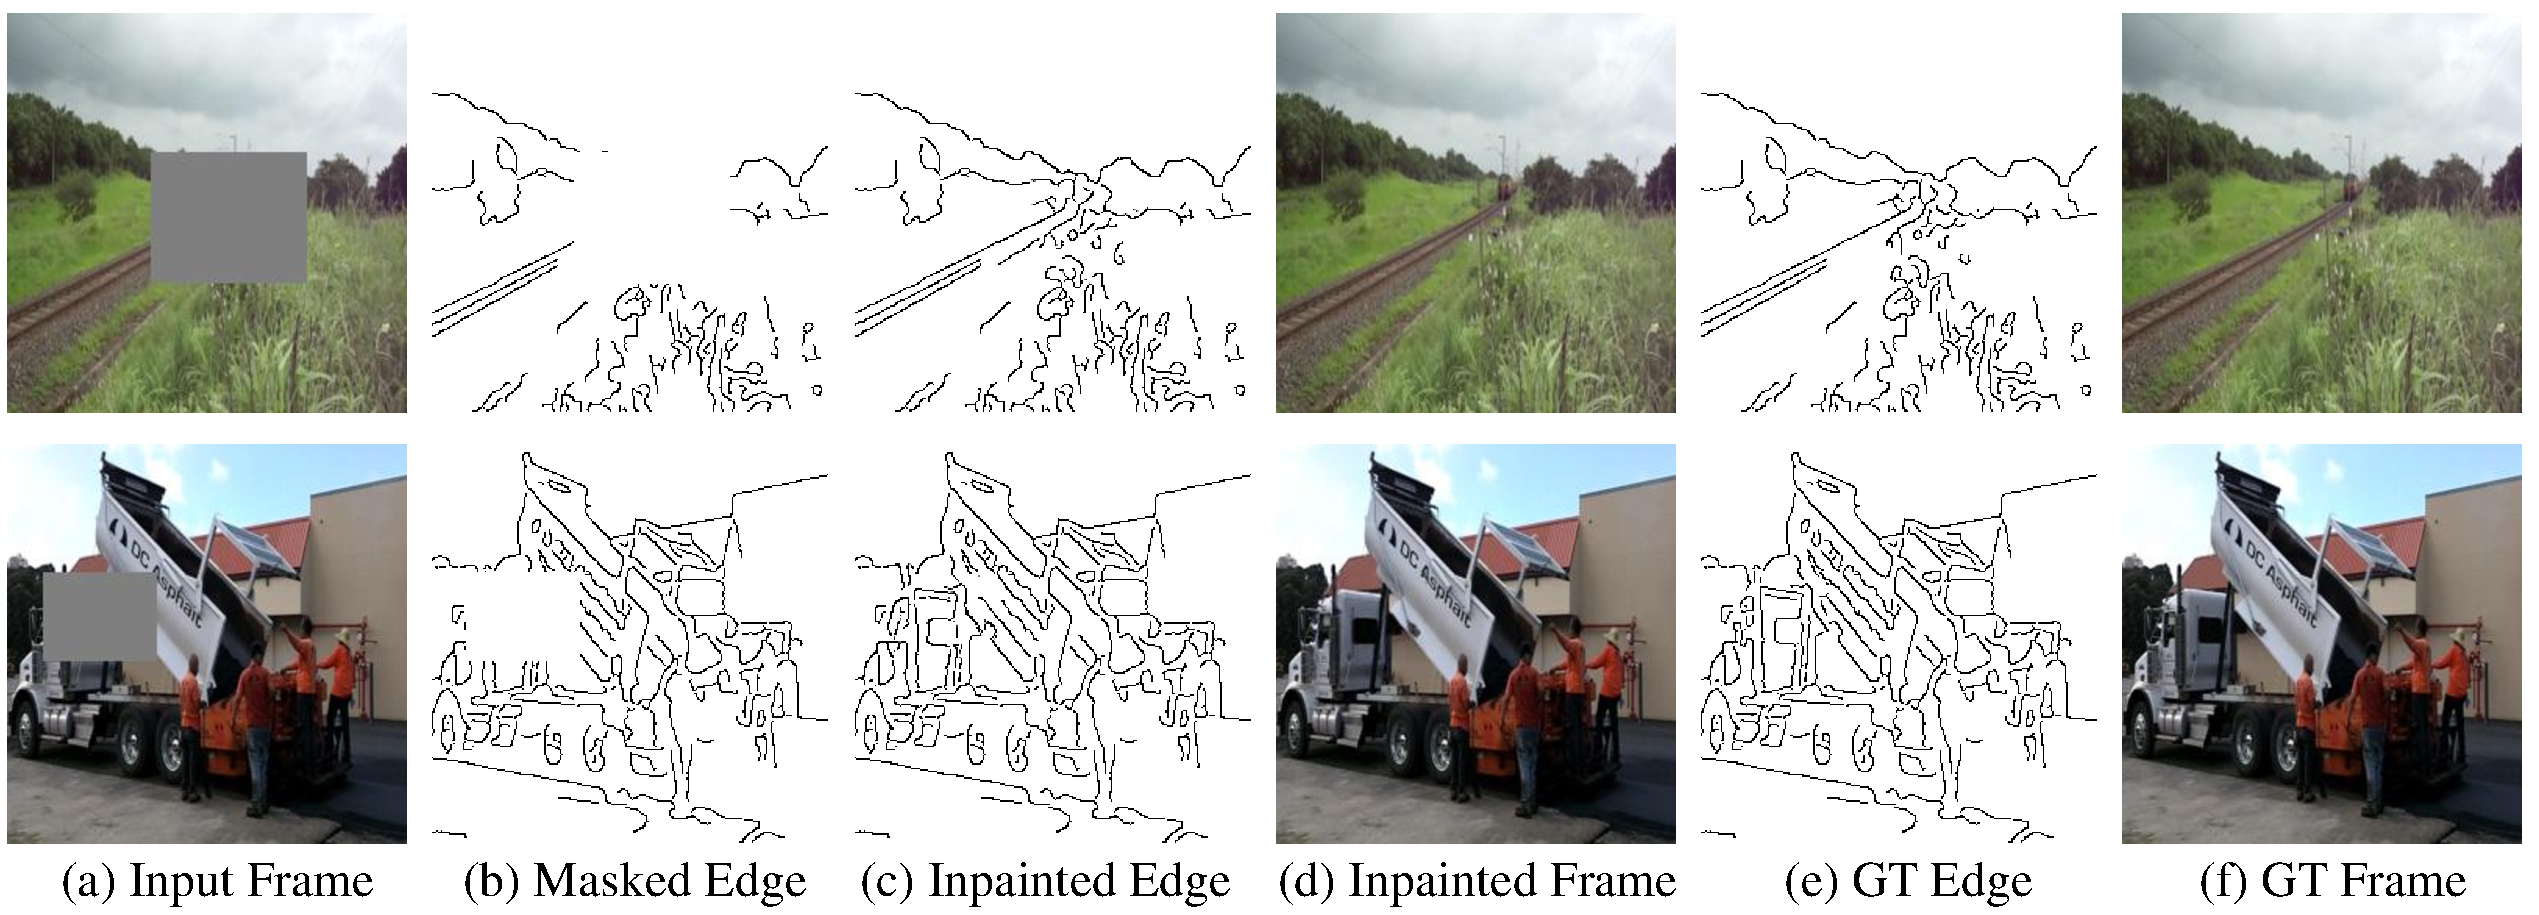
\includegraphics[width=0.97\columnwidth]{edgevis} % Reduce the figure size so that it is slightly narrower than the column. Don't use precise values for figure width.This setup will avoid overfull boxes. 
	\caption{Effects of structure guidance. By inpainting edge maps first and then filling texture, we generate more completed target structure. Clearer boundaries can be obtained using the structure attention module.}
	\label{edgevis}
\end{figure}

 
 
Comparing the four variants, `+ENet' brings large improvement over the baseline model.
It indicates that sparse edges provide effective structural guidance in video inpainting.
% which helps the network to predict accurate missing content.
When we further add SAM to `+ENet', extra improvement is obtained, demonstrating that the spatial correlation between edges and textures can be better embedded and absorbed by the texture inpainting network than simply feeding the completed edge maps as extra channels into TexNet.
%The above analyses prove that the edge clues are effective guidance in video inpainting, which helps the network to predict more accurate frames.
The inpainted edge map in Fig.~\ref{fig:coarse-fine} shows that ENet is capable of generating completed and detailed structure.
Fig.~\ref{edgevis} shows the results generated using the three variants. 
It is obvious that after introducing structure guidance, the inpainted frames become more visually pleasing with sharper object boundaries. 
Besides, the edge maps predicted by our method are reasonable and clear, which well represents the image structure and show the strong edge inpainting ability of ENet. 
Thus, it is crucial to explore structural details in video inpainting.




%\begin{figure}[t]
%	\centering
%	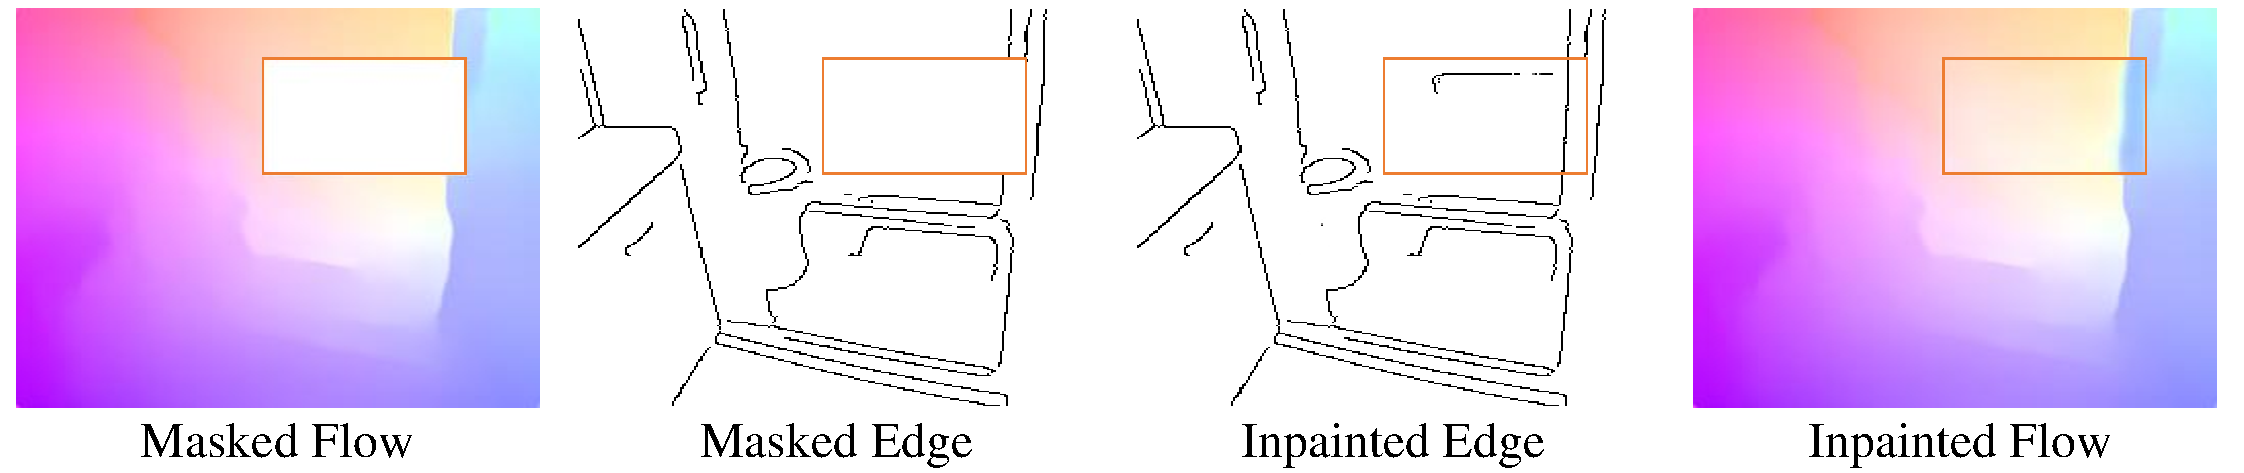
\includegraphics[width=1.0\columnwidth]{flowvis} % Reduce the figure size so that it is slightly narrower than the column. Don't use precise values for figure width.This setup will avoid overfull boxes. 
%	\caption{Visualized optical flow predicted by our method.}
%	\label{flowvis}
%\end{figure}
\begin{figure}[t]
	\centering
	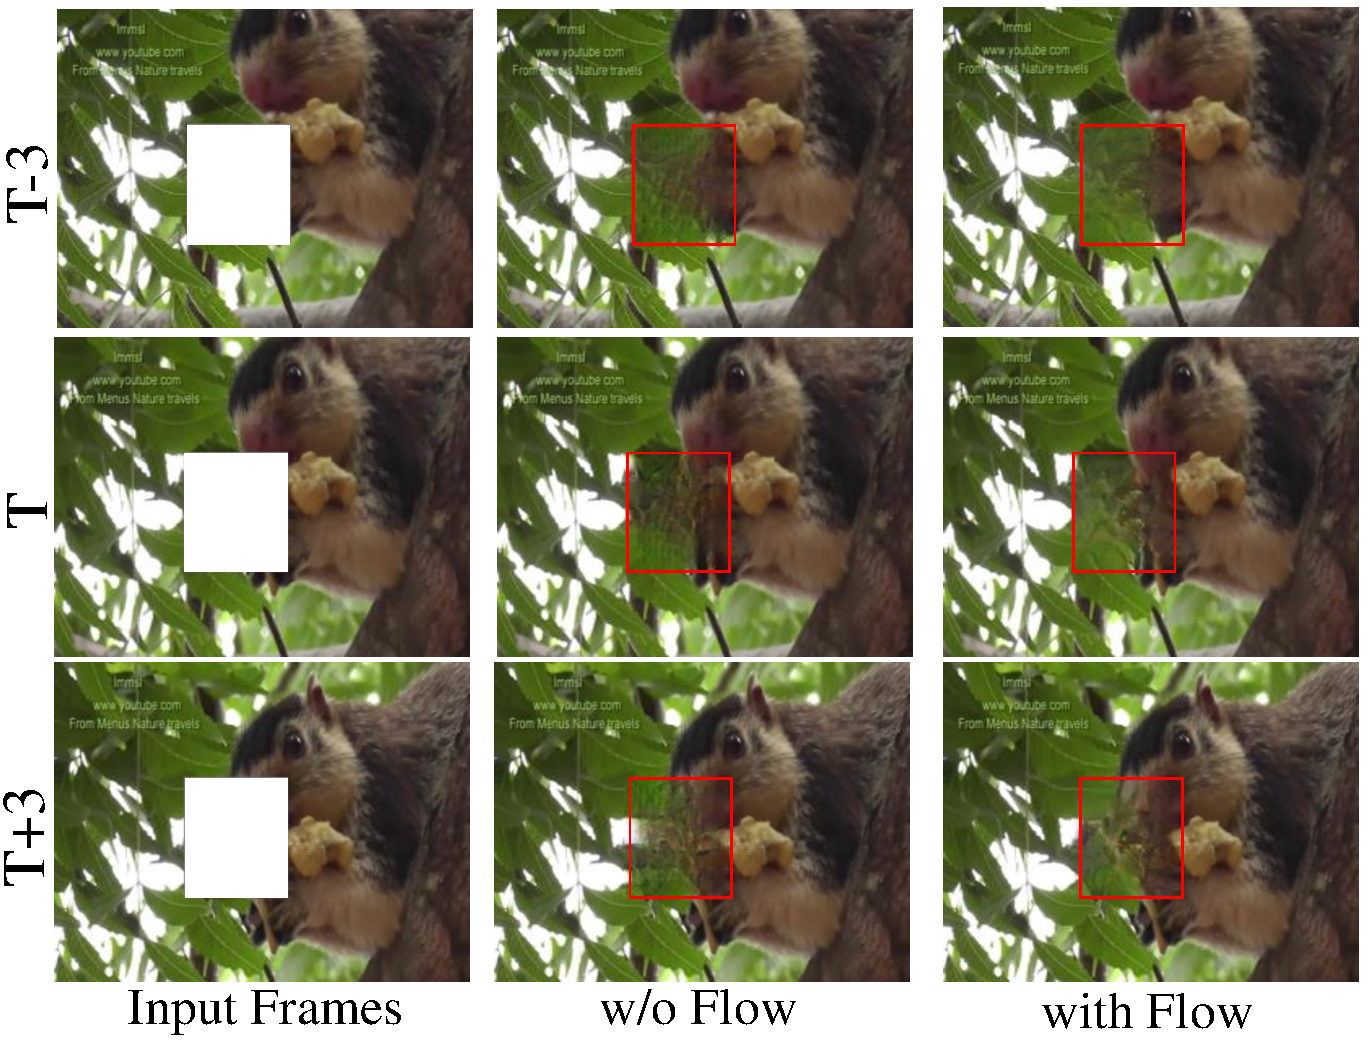
\includegraphics[width=0.9\columnwidth]{flow_vis} % Reduce the figure size so that it is slightly narrower than the column. Don't use precise values for figure width.This setup will avoid overfull boxes. 
	\caption{Inpainting results of three neighboring frames. With the flow assistance, the inpainting results are more temporally consistent without introducing image blurs. }
	\label{flow_vis}
\end{figure}

\subsubsection{Effect of Flow for Temporal Coherence.}

%Temporal coherence is an important factor in video inpainting. 
In our method, we utilize temporal information to smoothen artificial flickers via the developed flow-guided warping and temporal ensemble module. 
From Table~\ref{tab:sem}, we can see that the quantitative performance is slightly improved on all the three settings by adding the flow guidance. 
As shown in Fig.~\ref{flow_vis}, the synthesized contents in neighboring frames are more temporally consistent.
%and the color changes between neighboring frames become less obvious after employing flow.
The comparison can be better illustrated in the supplementary video.
Note that the performance gain from temporal ensemble is smaller than that from structure guidance in this paper.
The reason might be that our baseline model has certain ability to utilize complementary information of neighboring frames.
%Both the quantitative and qualitative results prove that the motion information is beneficial to temporal consistency as well as inpaitning.

 














 

